% !TeX root = ../main.tex
% Add the above to each chapter to make compiling the PDF easier in some editors.

\chapter{Background and Related Work}\label{chapter:related_work}

\section{Compressed Sensing}
Compressed sensing is a mathematical framework that enables the recovery of sparse signals from a reduced number of measurements \parencite{CompressedSensingIntro}.
The fundamental assumption behind compressed sensing is that the signal of interest is either sparse or compressible in some domain, meaning that most of its components are zero or near zero.
This property allows for the accurate reconstruction of signals even when the number of measurements is significantly smaller than the number of unknowns.

The standard compressed sensing formulation in the context of urban \gls{GHG} emission estimation, assuming that background emissions are known, is as follows:
\begin{equation}
    y = A x + \epsilon
\end{equation}
where $y \in \mathbb{R}$ represents the vector of measurements (e.g., atmospheric \gls{GHG} concentrations), $A \in \mathbb{R}^{m \times n}$ is the sensing matrix that models the relationship between the measurements and the emissions, $x \in \mathbb{R}^n$ is the unknown signal (i.e., the emission field), and $\epsilon$ is the noise term, capturing errors or uncertainties in the measurement process.
The sensing matrix $A$ represents the atmospheric transport of molecules and is derived from atmospheric transport models, such as STILT \parencite{STILT}.
A row in the sensing matrix $A$ corresponds to the vectorized sensitivity of a sensor to each grid cell.
Due to a lack of measurements compared to the number of unknowns and the high spatial correlation of these measurements, this problem is ill-posed.

There are many sparse reconstruction algorithms.
One of the most commonly used ones is the \gls{Lasso} \parencite{Lasso}, which solves the inverse problem by enforcing sparsity through L1-norm regularization.
Another prominent approach is \gls{BP} \parencite{BPDN}, which directly seeks the sparsest solution, and its variant \gls{BPDN} \parencite{BPDN}, which extends the model to handle noisy measurements.
These methods are crucial in emission estimation, where high-dimensional emission fields need to be recovered from a small number of measurements taken by atmospheric sensors.

\gls{Lasso} is a widely used method in compressed sensing due to its ability to enforce sparsity in the solution.
It achieves this by solving the following optimization problem:
\begin{equation}
    \min{\left( \norm{Ax -y }_2^2 + \alpha\norm{x}_1 \right)}
\end{equation}

In this formulation, $\norm{Ax -y }_2^2$ is the least-squares term that measures the difference between the observed measurements $y$ and the predicted measurements $Ax$.
In contrast, the L1-norm $\norm{x}_1$ promotes sparsity.
The parameter $\alpha$ controls the trade-off between the fit's accuracy and the solution's sparsity.
A larger $\alpha$ results in a sparser solution, whereas a smaller $\alpha$ allows for a closer fit to the observed data.
A smaller $\alpha$ may thus introduce non-zero components in $x$, leading to less sparsity.

\gls{BP} is another widely adopted algorithm for sparse reconstruction, particularly when the target is to find the sparsest possible solution that satisfies the measurement constraints $y = Ax$ exactly.
Basis pursuit solves the following optimization problem:
\begin{equation}
    \min \norm{x}_1 \quad \text{subject to} \quad  Ax = y
\end{equation}

Here, the objective is to minimize the L1-norm of the signal with the constraint of matching the predicted measurements $A x$ with the observed measurements $y$ exactly.
In contrast to \gls{Lasso}, \gls{BP} does not include a regularization term and instead focuses solely on finding the sparsest solution that satisfies the measurement equation.

\gls{BP} is ideal when the measurement process is noiseless, and the sensing matrix $A$ satisfies the \gls{RIP}, ensuring that different sparse signals remain distinguishable.
However, measurements are rarely noise-free in real-world applications, such as atmospheric \gls{GHG} monitoring, and thus $Ax = y$ cannot be enforced.

To address the limitations of basis pursuit in noisy environments, \gls{BPDN} introduces a tolerance for noise in the measurement process.
\gls{BPDN} modifies the original basis pursuit problem by allowing deviations from the exact measurement equation:
\begin{equation}
    \min \norm{x}_1 \quad \text{subject to} \quad  \norm{Ax -y}_2^2 \le \delta
\end{equation}

In this formulation, $\delta$ represents the allowable level of noise or error in the measurements.
Again, the L1-norm is minimized to promote sparsity in the signal, while the L2-norm ensures that the predicted measurements are close to the observed measurements within a defined noise threshold.
The parameter $\delta$ allows \gls{BPDN} to flexibly handle noisy data, making it more suitable for real-world scenarios, such as urban \gls{GHG} emission estimation, where measurement noise is inevitable due to sensor inaccuracies and atmospheric variability.

\gls{BPDN} strikes a balance between sparsity and measurement accuracy.
It is beneficial when the sensing matrix $A$ does not fully satisfy \gls{RIP}, or the measurement process involves significant noise.
By allowing for a controlled level of error, \gls{BPDN} can recover the sparse emission field without being overly sensitive to noise.
This means that \gls{BPDN} can tolerate a certain amount of noise in the measurements, ensuring robust solutions.

\section{Generative Models for Compressed Sensing}
\label{sec:cs_with_gen}

As mentioned, compressed sensing traditionally assumes that the underlying signals are sparse on some basis.
However, this assumption may only hold in some applications.
For instance, in urban emissions scenarios, while large point sources are often known or can be well-estimated, diffuse or area sources result in emission fields that are less sparse.
This lack of sparsity challenges the effectiveness of conventional compressed sensing techniques, potentially leading to reconstruction failures.

Generative models offer a promising alternative by relaxing the strict sparsity constraint \parencite{CSUsingAI}.
These models learn complex representations directly from data, circumventing the need for pre-specified sparse bases.
Recent advancements in fields such as medical imaging have successfully applied generative models to solve compressed sensing problems \parencite{ReviewCSUsingAI, CSUsingAI, SparseCSUsingAI}. %\parencite{jalal2021robust}).

In this thesis, we focus on the pioneering work by \textcite{CSUsingAI}, a framework that leverages generative models to improve upon classical compressed sensing techniques.
Their approach demonstrates that using neural networks trained to model the distribution of the underlying data can significantly enhance the performance of compressed sensing.

\subsection{Generative Models}\label{subsec:gen_models}

The framework developed by \textcite{CSUsingAI} primarily involves \gls{GAN} type models, including \gls{VAE}s \parencite{VAE} and \gls{GAN}s \parencite{GAN}.
Both \gls{VAE}s and \gls{GAN}s generate samples from lower-dimensional noise, transforming a latent variable $z \in \mathbb{R}^d$ into a data sample $x \in \mathbb{R}^n$ through a generator function $G: \mathbb{R}^d \to \mathbb{R}^n$.

\gls{VAE}s are probabilistic models that encode input data into a latent space and then decode it back to the original space.
They optimize a variational lower bound on the data likelihood, effectively learning a smooth latent space that captures the data distribution.

\gls{GAN}s consist of two neural networks, a generator $G$ and a discriminator $D$, trained in a minimax game.
The generator tries to produce data that is indistinguishable from real data, while the discriminator attempts to differentiate between real and generated data.
\gls{GAN}s are known for generating high-quality samples but can be challenging to train due to instability in the adversarial objectives.

While \gls{GAN}s often show superior quality in sample generation across various domains, their training instability \parencite{GAN} makes them less suitable for some applications.
Therefore, this thesis chooses \gls{VAE}s as the appropriate type of generative model due to their stability and structured latent space.

% Besides the work of \textcite{CSUsingAI}, there are many different approaches.
% For example, work using score-based or diffusion models (cite) in the context of medical imaging.
% Additionally, normalizing flows (cite) also show promising reults (cite).
% But since the goal of this thesis is not to compare individual ML based compressed sensing approaches, the focus lies on Bora et al. work.

\subsection{The Range of a Generator}

The range of a generator $G$ refers to the set of all possible outputs $G(z)$ as $z$ varies over the latent space $\mathbb{R}^d$ \parencite{CSUsingAI}.
This range represents the subset of the signal space $\mathbb{R}^n$ that the generative model can produce.
In the context of compressed sensing, the reconstruction is constrained to lie within this range, underscoring the importance of accurately capturing the true data distribution of the generative model.
Ideally, the generator captures emission field distribution perfectly, which means, in our case, that generated samples resemble emission flux fields.

\subsection{Compressed Sensing Framework}

The approach proposed by \textcite{CSUsingAI} integrates generative models into the compressed sensing reconstruction process.
Given a linear measurement model:
\begin{equation}
 y = A x + \epsilon
\end{equation}
where $A \in \mathbb{R}^{m \times n}$ is the sensing matrix, $x \in \mathbb{R}^n$ is the unknown signal (e.g., an emission field), $y \in \mathbb{R}^m$ represents the measurements, and $\epsilon$ denotes noise, the goal is to recover $x$ from $y$.

The key idea is to leverage a pre-trained generative model $G$ as an implicit prior for $x$.
In contrast to Bayesian inversion, this alleviates modeling errors due to a need for explicit priors.
The reconstruction problem is formulated as an optimization over the latent space:

\begin{equation}
 \min_{z}{\left( \norm{A G(z) - y}_2^2 + \gamma R(z) \right)}
\end{equation}
The generative model $G$ represents the range of possible signals, and the optimization seeks the latent vector $z$ that, when passed through $G$, produces a signal that matches the measurements $y$ as closely as possible.
The regularization term $R(z)$ encourages desirable properties in the solution, and $\gamma$ controls the strength of the regularization.
For instance, in the case of $z$ being Gaussian distributed, the regularization $R(z) = \norm{z}_2^2$ can be used.
The expression then represents a regularized optimization problem with Ridge (or Tikhonov) regularization \parencite{Ridge}.

Since $G$ is differentiable with respect to $z$, gradient-based optimization methods can be employed to solve the problem.
The optimization, seen in Figure \ref{fig:gen_solver}, seeks the latent vector $z^{\star}$ such that $G(z^{\star})$ best explains the measurements $y$.

\begin{figure}[htb]
    \centering
    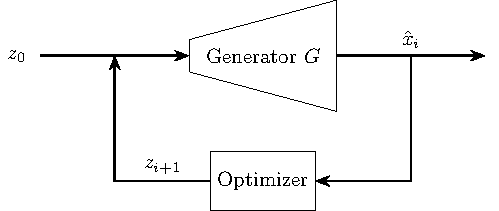
\includegraphics[width=0.75\textwidth]{figures/02_related_work/latent_variable_optimization/build/latent_variable_optimization.pdf}
    \caption{Compressed Sensing Framework Leveraging a Pre-trained Generator $G$ \parencite{CSUsingAI}}
    \label{fig:gen_solver}
\end{figure}

One limitation of above method is that the reconstructed signal $G(z^{\star})$ is confined strictly to the range of $G$.
This constraint may be too restrictive if $G$ does not perfectly capture the data distribution, leading to reconstruction errors.

\textcite{SparseCSUsingAI} proposed an extension that allows for sparse deviations from the generator's output to address this issue.
The modified optimization problem introduces an additional variable $s \in \mathbb{R}^n$ representing a sparse offset:

\begin{equation}
    \min_{z, s}{\left(\norm{s}_1 + \lambda \norm{A \left( G(z) + s \right) - y}_2^2 \right)}
    \label{eq:sparse_deviation}
\end{equation}
where $\norm{s}_1$ promotes sparsity in the offset $s$ and the parameter $\lambda$ balances the sparsity of $s$ with the fit to the measurements $y$.

The reconstructed signal is then given by $\hat{x} = G(z^\star) + s^\star$, where $z^\star$ and $s^\star$ are the solutions to the optimization problem in Equation \ref{eq:sparse_deviation}.

This extension allows the reconstruction to deviate slightly from the generator's range, accommodating components of the signal not captured by $G$, while maintaining overall consistency with the measurements and promoting sparsity in the deviations.

\section{Reconstruction Metrics}
Metrics are required to assess the quality of reconstructions.
In this thesis, we make use of two main metrics.
The first metric is inspired by \textcite{UrbanSparseReconstruction} and is the \gls{RE}.
Unlike the \gls{MSE} that is used as a reconstruction loss during training of the \gls{VAE}, the \gls{RE} is scale independent, making comparisons between cities consistent.
The \gls{RE} is defined as: 
\begin{equation}
    \text{RE}(x, \hat{x}) = \frac{\norm{x - \hat{x}}_2}{\norm{x}_2}
\end{equation}
where $\hat{x}$ is the vectorized reconstructed emission field, and $x$ the vectorized target emission field.

The second metric is the \gls{SSIM} \parencite{SSIM}.
This metric compares the structural information between two data fields by considering changes in local statistics such as mean, variance, and covariance.
Focusing on structural similarity provides a valuable complement to the \gls{RE}, which measures the relative error in terms of Euclidean distance.

\section{Research Questions}
This thesis aims at answering the following research questions:

\begin{itemize}
    \item To what extent can a \gls{VAE} capture meaningful low-dimensional representations of area-source emissions in urban inventories?
    \item How does the choice of latent space dimensionality in the \gls{VAE} impact the quality and accuracy of emission reconstructions?
    \item To what extent is the \gls{VAE} generalizable across diverse urban emission fields, or does it benefit from fine-tuning for specific cities?
    \item How effective is the \gls{VAE} in performing atmospheric inversion of area-source emissions, relative to established methods in compressed sensing?
\end{itemize}

While answering these questions, this thesis makes two major assumptions that impact the inverse problem.
First, like \textcite{UrbanSparseReconstruction}, we assume background emissions are known.
Second, like \textcite{JonesInversion}, we also assume large emitters, or point sources, are known.
